\documentclass{beamer}

\usepackage{listings}
\usepackage{xcolor}

\begin{document}

\section{Software Diversity}

Software diversity is a diverse field, and there is research focusing on different areas
with different goals in mind. However, what they all have in common is the that they are
exploring the potential benefits of engineering diversity within software development.
When talking about software diversity there are a few different classifications and goals
\cite[Section~1]{survey} which will be covered here.

Software diversity has a diverse (heh) set of goals ranging from fault-tolerance to re-usability
to security \cite{survey}.

\subsection{Managed Software diversity}

Managed software diversity is the notion of encouraging or controlling software diversity.

\subsubsection{Natural Diversity}

A lot of software with similar features naturally and spontaneously emerges from engineering
processes. There are a multitude of products from competing organizations that provide
the same function, for example routers, web browsers, compilers, database management systems
and firewalls. Natural diversity could also be something as simple as one program being
tunable by parameters to provide different functionality and performance \cite{survey}.

\subsubsection{Design Diversity}

Design diversity is the process of introducing diversity through the design process. For
example, \textit{N-version programming} is the approach where $N \geq 2$ functionality equivalent
programs are developed from the same specification. The point of this is that hopefully
it will result in a subset of the programs being free from bugs that another subset
might suffer from, thus creating a more fault tolerant system \cite{n-version}.

\subsection{Automated Software Diversity}

\textcite{survey} describes automated software diversity as \say{techniques for artificially
and automatically synthesizing diversity in software} \cite[\pno~8]{survey}. It is also
known as \textit{synthetic diversity} \cite{synthetic-diversity}. \say{Automated} is
referring to the fact that a human is not part of the diversification process, other than
having designed the framework \cite[Section~4]{survey}.

Automated diversity can characterize itself in different ways. A common approach is to
introduce some kind of randomness into software to break the otherwise deterministic behaviour
of most software. This can have several benefits, including security \cite{add-obfuscation}.
Randomization techniques are generally ways to either directly or indirectly create unique
execution of the same program \cite[Section~4.1]{survey}.

\subsubsection{Dynamic Randomization}

By introducing randomization at program run-time one can dynamically diversify the program
and introduce non-deterministic behaviour.

\textcite{os-randomization} randomizes the interface
between user space applications and the operating system by shuffling system call mappings,
changing library entry points and randomizing stack placement.

\textcite{mem-exploits} implements a source-to-source C-code transformer that randomizes
stack-resident variables, static data and individual functions (by introducing a level of
indirection to function calls).

\textcite{binary-stirring} introduces a technique they call \textit{stirring}, where
they accept input in the form of x86 binary code (without debug symbols, source code or
relocation information) and produce a new x86 binary file whose basics block addresses
are stirred and dynamically determined at program load-time.

Of course there are many more techniques and approaches but they will not be covered here.

\subsubsection{Static Randomization}

Static randomization creates diversity at compile time by generating several versions of the
same program that are functionally equivalent but semantically different. This can be done
in a variety of ways including but not limited to: exploiting NOP (no operation) instructions,
instruction set randomization, reversing the stack, stack frame padding,
and obfuscation (register randomization, variable reordering etc)
\cite{survey, compiler-generated-sw-div},

This thesis will focus on static, compiler generated randomization. Just as for dynamic
randomization, static randomization's current focus is security. The key insight is that
while the same source code always yields the same binary in the current climate, the compiler
takes a lot of decisions based on heuristics when reaching this concluding binary (see \ref{sec:llvm}).
It is even the case that those decisions might be flawed and that a different heuristic
might have yielded a better result (see \ref{sec:unison}). Not only does this indicate
that there is room for improvements in present-day compilers, but it also a huge potential
for automated software diversity. For example, if we compile:

\lstinputlisting[label={src:vec-add},caption=A C++ function for adding two vector values,
language=C++,tabsize=2,frame=single,breaklines=true, showstringspaces=false,
backgroundcolor=\color{lightgray}]{background/software-diversity/examples/vec_add.cpp}

we can generate multiple different binaries simply by using multiple different compilers.
Here are two examples using gcc and clang (with -Ofast):

\lstinputlisting[caption=Assembly emitted by gcc for listing \ref{src:vec-add},tabsize=2,
frame=single, breaklines=true,showstringspaces=false,backgroundcolor=\color{lightgray}]
{background/software-diversity/examples/gcc_vec_add.s}

\lstinputlisting[caption=Assembly emitted by clang for listing \ref{src:vec-add},tabsize=2,
frame=single, breaklines=true,showstringspaces=false,backgroundcolor=\color{lightgray}]
{background/software-diversity/examples/clang_vec_add.s}

Even though this function is very small the resulting assembly is very different. In this
case the assembly produced by gcc is basically garbage (in terms of optimizations)
compared to the one produced by clang (a difference of 20 instructions) but nonetheless
they are two functionally equal but semantically different binaries. This is to emphasise
that software diversity is not a foreign concept, but rather very commonly occuring.

There are ways to deploy and steer this inherent diversity. \textcite{compiler-generated-sw-div}
have explored two approaches to this. One where they implement a diversification engine for
an App Store (such as Apple's App Store or Google Play Store) that automatically generates
a unique binary for every download. The other approach is to run multiple variants of the
same program at the same time in parallel and verifying that their behaviour is correct.
Both of these approaches can make use of more or less all previously mentioned diversity
techniques, both dynamic and static.

We will explore the diversity potential in integrated instruction scheduling and register
allocation by using a tool that functions by combinatorial exploration of binary programs
that potentially represents the input source code (\ref{sec:llvm} and \ref{sec:unison}).
In other words, it compiles the code by working out possible binary representations of the
program and then iteratively verifying them to find a solution.

\subsection{Why bother?}
\subsubsection{Return Oriented Programming}
Return oriented programming hijacks the call stack to divert control flow in a program. It
works by overwriting the return address of a function call to execute instruction sequences
outside the intended order. By carefully choosing these sequences (called gadgets) an adversary
can perfor arbitrary operations. \textcite{rop} not only introduced this technique
but also showed that more or less all binaries contain enough of these gadgets to execute
arbitrary code (such as opening a shell).

The attack is mainly about identifying these gadgets, construction a sequence of
gadgets to execute the sought-after code and construction a payload which somehow hijacks
the control flow of the program to execute this sequence of gadgets. If we can somehow
break these gadgets then the payload will be useless. However, as \textcite{rop} showed
it is not practically impossible to break all gadgets. What we can do, however, is diversify
our binaries. By compiling several different binaries who all have different instruction
sequences we break these gadgets, and thus make attacking all versions of our program
a lot more resource heavy. As it stands now by construction a payload on one binary you can
attack all of them. If we diversify, that payload only works on the specific binary it was
constructed for.

\textcite{large-scale-automated} explored two static compiler techniques to break these
gadgets, NOP insertion and randomizing instruction scheduling. While they found that their
techiques worked very well they both rely on randomness. More specifically they insert
NOP randomly in the code and randomize the instruction schedule. Both of these techniques
offers no \textit{guarantees} that the resulting binaries will the diverse enough and they
also introduce some overhead when executing the binaries (albeit small).


%return oriented programming: https://www.informatik.tu-darmstadt.de/fileadmin/user_upload/Group_TRUST/PubsPDF/readactor.pdf
% Show gadgets in previously emitted assembly (vec_add)


\begin{frame}
	\frametitle{LLVM}
	LLVM is an umbrella project that provides a collection of tools for developing low-level
	toolchains, e.g assemblers, compilers, debuggers, linkers etc. 
\end{frame}

\begin{frame}
	\frametitle{Three-Phase Design}
	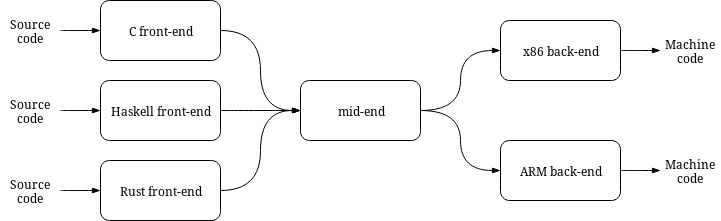
\includegraphics[width=11cm]{../background/llvm/figures/three_phase_compiler}
\end{frame}

\begin{frame}
	\frametitle{The Backend}

	\begin{itemize}
		\item instruction selection
		\item instruction scheduling
		\item register allocation
		\item code layout optimization
		\item assembly code emission
	\end{itemize}

\end{frame}

\begin{frame}
	\frametitle{LLVM Machine Specific Representation}

	\begin{itemize}
		\item	In-memory data structures
		\item	Can be serialized into \textit{Machine Intermediate Representation} (YAML).
	\end{itemize}

\end{frame}

\begin{frame}
	\frametitle{LLVM MIR}

	\lstinputlisting[language=C,tabsize=2,frame=single,breaklines=true,showstringspaces=false]
	{../background/llvm/examples/factorial.c}

\end{frame}


\begin{frame}
	\frametitle{LLVM MIR}

	\lstinputlisting[basicstyle=\tiny,tabsize=2,frame=single,breaklines=true,showstringspaces=false]
	{../background/llvm/examples/factorial.mir}

	Courtesy of the Unison documentation.
\end{frame}

\begin{frame}
	\frametitle{Problems}

	\begin{itemize}
		\item Treating each task a distinct steps
		\item Machine specific problems
	\end{itemize}
\end{frame}


\begin{frame}
	\frametitle{Constraint Programming}
	Also called \textit{Combinatorial Optimization}.

	\vspace{1cm}

	A programming paradigm where you are describing the charactersitics of a solution
	rather than the steps needed to reach a solution.
\end{frame}

\begin{frame}
	\frametitle{Solving a Problem in 3 easy steps!}

	\begin{enumerate}
		\item Identifying variables and corresponding domains
		\item Determining Constraints
		\item Choosing a search heuristic
	\end{enumerate}
\end{frame}

\begin{frame}
	\frametitle{Identifying Variables}
	$SEND + MOST = MONEY$
	
	\vspace{0.5cm}
	\noindent
	$S \in \{0, 1, 2, 3, 4, 5, 6, 7, 8, 9\}$ \\
	$E \in \{0, 1, 2, 3, 4, 5, 6, 7, 8, 9\}$ \\
	$N \in \{0, 1, 2, 3, 4, 5, 6, 7, 8, 9\}$ \\
	$D \in \{0, 1, 2, 3, 4, 5, 6, 7, 8, 9\}$ \\
	$M \in \{0, 1, 2, 3, 4, 5, 6, 7, 8, 9\}$ \\
	$O \in \{0, 1, 2, 3, 4, 5, 6, 7, 8, 9\}$ \\
	$T \in \{0, 1, 2, 3, 4, 5, 6, 7, 8, 9\}$ \\
	$Y \in \{0, 1, 2, 3, 4, 5, 6, 7, 8, 9\}$
\end{frame}

\begin{frame}
	\frametitle{Determining Constraints}
	Relationship between variables.

	\begin{tabular}{cccccc}
		& & $1000 * S$ & $100 * E$ & $10 * N$ & $D$ \\
		+ &	& $1000 * M$ & $100 * O$ & $10 * S$ & $T$ \\
		\hline
		& $10000 * M$ & $1000 * O$ & $100 * N$ & $10 * E$ & $Y$
	\end{tabular}

\end{frame}

\begin{frame}
	\frametitle{Choosing a Search Heuristic}
	Search heuristic is a fancy word for "how we want to guess".
	
	\vspace{1cm}

	When we can no longer shrink domains but there are still multiple possibilities we guess.
\end{frame}

\begin{frame}
	\frametitle{Propagating and Searching}
	\begin{columns}
		\begin{column}{0.5\textwidth}
			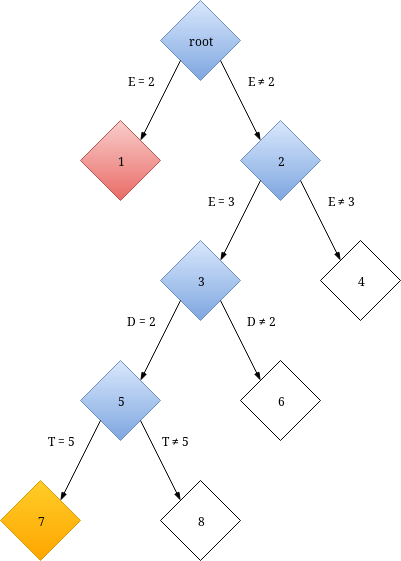
\includegraphics[width=6cm]{../background/constraint-programming/figures/constraint_first_solution}
		\end{column}

		\tabcolsep=0.11cm
		\begin{column}{0.5\textwidth}
			\begin{tabular}{c|c|c|c|c|c}
				Variable & root & 2 & 3 & 5 & 7 \\
				\hline
				S & 9 & 9 & 9 & 9 & 9 \\
				E & 2..7 & 3..7 & 3 & 3 & 3 \\
				N & 3..8 & 4..8 & 4 & 4 & 4 \\
				D & 2..8 & 2..8 & 2,5,6 & 2 & 2 \\
				M & 1 & 1 & 1 & 1 & 1 \\
				O & 0 & 0 & 0 & 0 & 0 \\
				T & 2..8 & 2..8 & 2,5,6 & 5,6 & 5 \\
				Y & 2..8 & 2..8 & 5..8 & 7,8 & 7 \\
			\end{tabular}

		\end{column}
	\end{columns}
\end{frame}

\begin{frame}
	\frametitle{Optimizing}
	Unexplored options

	\vspace{1cm}

	For further combinations to be considered a solution we require $MONEY$ to map to a bigger integer.

	\vspace{1cm}
	
	\centering
	\begin{tabular}{c|c|c|c|c|c|c|c|c}
		S & E & N & D & M & O & T & Y & MONEY \\
		\hline
		9 & 7 & 8 & 2 & 1 & 0 & 4 & 6 & 10876 \\
	\end{tabular}

\end{frame}


\section{Unison}
\label{sec:unison}

Unison is an open-source\footnote{\url{https://github.com/unison-code/unison}},
potentially optimal tool that performs integrated register allocation and instruction
scheduling using constraint programming. It can be used as an alternative or complement to
the algorithms currently in place by compilers such as GCC and LLVM. In particular there
already exists a driver for LLVM which accept input in the form of LLVM MIR \cite{unison-docs}.

\subsection{Constraint Programming}

Constraint programming is a programming paradigm for solving combinatorial problems.
By declaring all variables possible values and their \textit{constraints}, the relationship
between them when part of a solution, a \textit{constraint solver} can search the solution
space and find an assignment of variables to values that is consistent with the constraints.
A constraint solver effectively explores different possible combinations systematically,
by a potentially incomplete local inference (also known as \textit{constraint propagation})
or more commonly a combination of the two \cite{handbook-constraint-programming}.

Currently the only constraint solver supported by Unison is Gecode\footnote{\url{www.gecode.org}}
\cite{unison-docs}, which is a constraint solver that interleaves system search algorithms
search with constraint propagation\cite{MPG}.

When propagating constraints the Gecode solver searches all variable's domains and removes
variables that in conflict with the constraints\cite[Section~23.1]{MPG}. For example,
given two variables (and their corresponding domains) $x \in {0,1,2}$ and $y \in {0,1,2}$
and the constraint $x > y$ constraint propagation can determine that $x \in {1, 2}$ and
$y \in {0, 1}$ are the only combinations consistent with the constraint.

When constraint propagation is finished there are three possible states:

\begin{enumerate}
	\item One or more domains could be empty, proving that no solution exists.
	\item	All domains could be of size 1, indicating that there exists only one possible
		value for every variable, and thus we have found a solution.
	\item One or more variables have multiple values in their domain.
\end{enumerate}

For situation (1) and (2), either a solution is found or we have proven that a solution
does not exist (within the local search space).

In the latter situation (3) the Gecode constraint solver splits a variable's domain into
two or more subsets, creating a \textit{search tree} where each \textit{branch} represents
reducing the variable's domain to a particular subset \cite[Section~8]{MPG}. By commiting
to a branch the constraint solver can once again perform constraint propagation and repeat
the process. However, if \textit{branching} has taken place and the solver reaches
situation (1) it can go back up the tree and explore a different branch. If situation (2)
is reached it can still backtrack but with the added option of adding more constraints
based on the newly found solution. Constraining based on previously found solutions in the
search tree is done with the \textit{branch-and-bound} search engine\cite[Section~9]{MPG}
in Gecode.

\textit{Branch and bound} is an efficient strategy to find the optimal solution to a
combinatorial problem which in essence constitutes comparing potential solutions to the
currently best found solution, choosing the better of the two\cite{BaB}. We will adopt a
similar strategy, but instead of constraining solutions to be better we will require them
to be \textit{different}. In addition, no solutions will be discarded.

\subsection{Unison}


Unison models the problems of register allocation and instruction scheduling as a single
constraint-satisfaction problem and solves them simultaneously \cite{unison-docs,reg-alloc-inst-sched-uni}.

Unison's key properties are that it introduces \textit{optional copies} and
\textit{alternative temporaries} \cite{reg-alloc-inst-sched-uni}. This allows Unison to
support different register allocation decision and perform otherwise unreachable optimizations
\cite{reg-alloc-inst-sched-uni, comb-spill}.


\begin{frame}
	\frametitle{Unison for SW Diversity}

	Can explore the entire diversity space.

	\vspace{0.5cm}

	We do not need to rely on randomness.

	\vspace{0.5cm}

	Possibly no overhead (compared to LLVM).
\end{frame}

\begin{frame}
	\frametitle{MIR to Machine Code}

	Is the mapping deterministic?

	\vspace{0.5cm}

	Perhaps it's enough to say that different MIR means different machine code?
\end{frame}

\end{document}
